% ============================================================================
% CHAPTER 5: MULTI-LAYER PERCEPTRONS
% ============================================================================

\chapter{Multi-Layer Perceptrons}
\label{ch:mlp}

% ============================================================================
% OVERVIEW
% ============================================================================

\section{Chapter Overview}

This chapter introduces \textbf{Multi-Layer Perceptrons (MLPs)}---neural networks with multiple layers that can solve non-linearly separable problems. We establish formal definitions of network depth, layers, and notation that will be used throughout our study of deep learning.

\textbf{Learning Objectives:}
\begin{itemize}
    \item Understand why multiple layers are needed
    \item Define depth and layers using graph theory
    \item Master standard neural network notation
    \item Trace information flow through deep networks
    \item Understand the matrix formulation of neural networks
\end{itemize}

% ============================================================================
% WHY MULTIPLE LAYERS?
% ============================================================================

\section{The Need for Multiple Layers}

\subsection{The XOR Revisited}

Recall that a single perceptron cannot solve XOR because it's not linearly separable. However, XOR \textit{can} be expressed as a combination of simpler functions:

\[
\text{XOR}(x_1, x_2) = \text{AND}(\text{OR}(x_1, x_2), \text{NAND}(x_1, x_2))
\]

This suggests that by \textbf{combining multiple neurons}, we can solve problems that individual neurons cannot.

\begin{center}
\begin{tikzpicture}[
    input/.style={circle, draw, fill=blue!20, minimum size=0.8cm},
    neuron/.style={circle, draw, fill=yellow!30, minimum size=0.8cm},
    output/.style={circle, draw, fill=red!20, minimum size=0.8cm}
]
    % Inputs
    \node[input] (x1) at (0, 1.5) {$x_1$};
    \node[input] (x2) at (0, -1.5) {$x_2$};
    
    % Hidden layer
    \node[neuron] (or) at (3, 1) {OR};
    \node[neuron] (nand) at (3, -1) {NAND};
    
    % Output
    \node[output] (and) at (6, 0) {AND};
    
    % Connections
    \draw[-Stealth] (x1) -- (or);
    \draw[-Stealth] (x1) -- (nand);
    \draw[-Stealth] (x2) -- (or);
    \draw[-Stealth] (x2) -- (nand);
    \draw[-Stealth] (or) -- (and);
    \draw[-Stealth] (nand) -- (and);
    
    % Labels
    \node[above] at (6, 0.5) {XOR};
\end{tikzpicture}
\end{center}

\begin{bluebox}[Key Insight: Hierarchical Computation]
Just as the visual cortex processes information in layers (edges $\rightarrow$ shapes $\rightarrow$ objects $\rightarrow$ scenes), neural networks can build complex representations by composing simpler ones layer by layer.
\end{bluebox}

% ============================================================================
% GRAPH THEORY FOUNDATIONS
% ============================================================================

\section{Neural Networks as Graphs}

\subsection{Directed Acyclic Graphs (DAGs)}

Neural networks can be represented as \textbf{directed acyclic graphs (DAGs)}:

\begin{itemize}
    \item \textbf{Nodes}: Neurons (computational units)
    \item \textbf{Edges}: Weighted connections (parameters)
    \item \textbf{Directed}: Information flows in one direction
    \item \textbf{Acyclic}: No loops or cycles
\end{itemize}

\begin{definitionbox}[Source and Sink Nodes]
\begin{itemize}
    \item \textbf{Source nodes}: Nodes with no incoming edges (input layer)
    \item \textbf{Sink nodes}: Nodes with no outgoing edges (output layer)
\end{itemize}
\end{definitionbox}

\subsection{Defining Depth}

\begin{definitionbox}[Depth of a Neural Network]
The \textbf{depth} of a neural network is the number of edges on the \textit{longest path} from any source node to any sink node.
\[
\text{depth} = \max_{\text{paths } s \to t} (\text{number of edges on path})
\]
where $s$ is a source and $t$ is a sink.
\end{definitionbox}

\begin{examplebox}[Computing Depth]
Consider a network with:
\begin{itemize}
    \item 3 input nodes (layer 0)
    \item 4 hidden nodes (layer 1)
    \item 4 hidden nodes (layer 2)
    \item 2 output nodes (layer 3)
\end{itemize}

The longest path has $3$ edges (input $\to$ hidden1 $\to$ hidden2 $\to$ output).

Therefore, the network has \textbf{depth 3}.
\end{examplebox}

\subsection{What Makes a Network ``Deep''?}

\begin{definitionbox}[Deep Network]
A neural network is called \textbf{deep} if its depth is greater than 2.
\[
\text{Deep network} \Leftrightarrow \text{depth} > 2
\]
\end{definitionbox}

Networks with depth 2 (one hidden layer) are sometimes called ``shallow'' networks.

\subsection{Defining Layers}

\begin{definitionbox}[Layer Assignment]
A neuron belongs to \textbf{layer $k$} if the maximum number of edges from any source node to that neuron is $k$.
\[
\text{layer}(n) = \max_{\text{paths } s \to n} (\text{number of edges})
\]
\end{definitionbox}

This means:
\begin{itemize}
    \item Input nodes are in layer 0
    \item All neurons reachable in exactly $k$ edges are in layer $k$
    \item Output nodes are in layer $L$ (the final layer)
\end{itemize}

% ============================================================================
% MLP NOTATION
% ============================================================================

\section{Standard Neural Network Notation}

\subsection{Network Structure}

Consider a network with:
\begin{itemize}
    \item $L$ layers (not counting input)
    \item $n^{[l]}$ neurons in layer $l$
\end{itemize}

\begin{center}
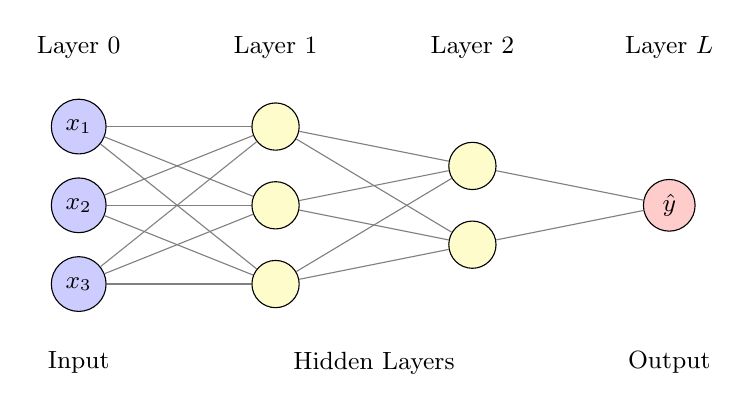
\begin{tikzpicture}[
    input/.style={circle, draw, fill=blue!20, minimum size=0.6cm, font=\small},
    hidden/.style={circle, draw, fill=yellow!20, minimum size=0.6cm, font=\small},
    output/.style={circle, draw, fill=red!20, minimum size=0.6cm, font=\small}
]
    % Layer labels
    \node at (0, 2.5) {\small Layer 0};
    \node at (2.5, 2.5) {\small Layer 1};
    \node at (5, 2.5) {\small Layer 2};
    \node at (7.5, 2.5) {\small Layer $L$};
    
    % Input layer
    \node[input] (x1) at (0, 1.5) {$x_1$};
    \node[input] (x2) at (0, 0.5) {$x_2$};
    \node[input] (x3) at (0, -0.5) {$x_3$};
    
    % Hidden layer 1
    \node[hidden] (h11) at (2.5, 1.5) {};
    \node[hidden] (h12) at (2.5, 0.5) {};
    \node[hidden] (h13) at (2.5, -0.5) {};
    
    % Hidden layer 2
    \node[hidden] (h21) at (5, 1) {};
    \node[hidden] (h22) at (5, 0) {};
    
    % Output
    \node[output] (y) at (7.5, 0.5) {$\hat{y}$};
    
    % Connections (simplified)
    \foreach \i in {x1, x2, x3} {
        \foreach \j in {h11, h12, h13} {
            \draw[gray, thin] (\i) -- (\j);
        }
    }
    \foreach \i in {h11, h12, h13} {
        \foreach \j in {h21, h22} {
            \draw[gray, thin] (\i) -- (\j);
        }
    }
    \foreach \i in {h21, h22} {
        \draw[gray, thin] (\i) -- (y);
    }
    
    % Labels below
    \node at (0, -1.5) {\small Input};
    \node at (3.75, -1.5) {\small Hidden Layers};
    \node at (7.5, -1.5) {\small Output};
\end{tikzpicture}
\end{center}

\subsection{Weight Matrix Notation}

\begin{definitionbox}[Weight Matrix $\mat{W}^{[l]}$]
The weight matrix $\mat{W}^{[l]}$ contains weights connecting layer $l-1$ to layer $l$:
\[
\mat{W}^{[l]} \in \R^{n^{[l]} \times n^{[l-1]}}
\]

Element $W_{ij}^{[l]}$ is the weight from neuron $j$ in layer $l-1$ to neuron $i$ in layer $l$.
\end{definitionbox}

\textbf{Indexing convention}: The destination neuron index comes first (row), then the source neuron index (column). This facilitates matrix multiplication in the forward pass.

\subsection{Bias Vector Notation}

\begin{definitionbox}[Bias Vector $\vect{b}^{[l]}$]
The bias vector for layer $l$:
\[
\vect{b}^{[l]} \in \R^{n^{[l]}}
\]

Element $b_i^{[l]}$ is the bias for neuron $i$ in layer $l$.
\end{definitionbox}

\subsection{Activation Notation}

\begin{definitionbox}[Pre-activation and Activation]
For layer $l$:
\begin{itemize}
    \item \textbf{Pre-activation} (before nonlinearity):
    \[
    \vect{a}^{[l]} = \mat{W}^{[l]} \vect{h}^{[l-1]} + \vect{b}^{[l]}
    \]
    
    \item \textbf{Activation} (after nonlinearity):
    \[
    \vect{h}^{[l]} = \sigma(\vect{a}^{[l]})
    \]
\end{itemize}

Note: $\vect{h}^{[0]} = \vect{x}$ (the input).
\end{definitionbox}

\subsection{Summary of Notation}

\begin{center}
\renewcommand{\arraystretch}{1.3}
\begin{tabular}{|c|c|c|}
\hline
\textbf{Symbol} & \textbf{Meaning} & \textbf{Dimensions} \\ \hline
$L$ & Number of layers (excluding input) & Scalar \\ \hline
$n^{[l]}$ & Number of neurons in layer $l$ & Scalar \\ \hline
$\mat{W}^{[l]}$ & Weight matrix for layer $l$ & $n^{[l]} \times n^{[l-1]}$ \\ \hline
$\vect{b}^{[l]}$ & Bias vector for layer $l$ & $n^{[l]} \times 1$ \\ \hline
$\vect{a}^{[l]}$ & Pre-activation (linear output) & $n^{[l]} \times 1$ \\ \hline
$\vect{h}^{[l]}$ & Activation (hidden output) & $n^{[l]} \times 1$ \\ \hline
$\vect{h}^{[0]} = \vect{x}$ & Input & $n^{[0]} \times 1$ \\ \hline
$\vect{h}^{[L]} = \hat{\vect{y}}$ & Network output & $n^{[L]} \times 1$ \\ \hline
\end{tabular}
\end{center}

% ============================================================================
% FORWARD PROPAGATION
% ============================================================================

\section{Forward Propagation in MLPs}

\subsection{The Algorithm}

\begin{tcolorbox}[title=Forward Propagation Algorithm]
\textbf{Input}: $\vect{x}$ (input features), $\{\mat{W}^{[l]}, \vect{b}^{[l]}\}_{l=1}^{L}$ (parameters)

\textbf{Output}: $\hat{\vect{y}}$ (prediction)

\begin{enumerate}
    \item Set $\vect{h}^{[0]} = \vect{x}$
    \item For $l = 1, 2, \ldots, L$:
    \begin{enumerate}
        \item Compute pre-activation: $\vect{a}^{[l]} = \mat{W}^{[l]} \vect{h}^{[l-1]} + \vect{b}^{[l]}$
        \item Apply activation: $\vect{h}^{[l]} = \sigma(\vect{a}^{[l]})$
    \end{enumerate}
    \item Return $\hat{\vect{y}} = \vect{h}^{[L]}$
\end{enumerate}
\end{tcolorbox}

\subsection{Matrix Formulation}

For a batch of $m$ examples, we can process all inputs simultaneously:

\[
\mat{H}^{[0]} = \mat{X} \in \R^{n^{[0]} \times m}
\]

\[
\mat{A}^{[l]} = \mat{W}^{[l]} \mat{H}^{[l-1]} + \vect{b}^{[l]} \mathbf{1}^\top
\]

\[
\mat{H}^{[l]} = \sigma(\mat{A}^{[l]})
\]

This matrix formulation enables efficient computation on GPUs.

\subsection{Python Implementation}

\begin{lstlisting}[language=Python, caption=Forward Propagation]
import numpy as np

def forward_pass(X, weights, biases, activation=sigmoid):
    """
    Compute forward pass through an MLP.
    
    Args:
        X: Input data (n_features, n_samples)
        weights: List of weight matrices [W1, W2, ..., WL]
        biases: List of bias vectors [b1, b2, ..., bL]
        activation: Activation function
    
    Returns:
        List of activations [h0, h1, ..., hL]
    """
    H = [X]  # h0 = X
    
    for l in range(len(weights)):
        # Pre-activation
        A = weights[l] @ H[l] + biases[l]
        
        # Activation
        H.append(activation(A))
    
    return H
\end{lstlisting}

% ============================================================================
% REPRESENTATIONAL POWER
% ============================================================================

\section{Representational Power}

\subsection{Universal Approximation Theorem}

A profound result in neural network theory:

\begin{theorembox}[Universal Approximation Theorem (Informal)]
A feedforward neural network with a single hidden layer containing a finite number of neurons can approximate any continuous function on compact subsets of $\R^n$, under mild assumptions on the activation function.
\end{theorembox}

This means MLPs are \textbf{universal function approximators}---they can theoretically represent any function we might want to learn.

\begin{importantbox}[Existence vs. Learnability]
The Universal Approximation Theorem only guarantees \textit{existence} of a good network. It says nothing about:
\begin{itemize}
    \item How many neurons are needed
    \item Whether we can \textit{find} the right weights through training
    \item Whether the solution will generalize to new data
\end{itemize}

In practice, deeper networks with fewer neurons per layer often work better than shallow, wide networks.
\end{importantbox}

\subsection{Why Depth Helps}

Deep networks have advantages over shallow ones:

\begin{enumerate}
    \item \textbf{Hierarchical features}: Each layer can learn increasingly abstract representations
    \item \textbf{Efficiency}: Some functions require exponentially fewer neurons when represented with depth
    \item \textbf{Modularity}: Lower layers can be reused for different tasks (transfer learning)
\end{enumerate}

% ============================================================================
% SUMMARY
% ============================================================================

\section{Chapter Summary}

\begin{itemize}
    \item \textbf{Multiple layers} enable solving non-linearly separable problems like XOR.
    
    \item Neural networks are \textbf{directed acyclic graphs (DAGs)} with source (input) and sink (output) nodes.
    
    \item \textbf{Depth} = number of edges on longest path from input to output. Deep networks have depth $> 2$.
    
    \item \textbf{Standard notation}:
    \begin{itemize}
        \item $\mat{W}^{[l]}$: Weight matrix for layer $l$
        \item $\vect{b}^{[l]}$: Bias vector for layer $l$
        \item $\vect{a}^{[l]}$: Pre-activation, $\vect{h}^{[l]}$: Activation
    \end{itemize}
    
    \item \textbf{Forward propagation}: Sequential computation through layers:
    \[
    \vect{a}^{[l]} = \mat{W}^{[l]} \vect{h}^{[l-1]} + \vect{b}^{[l]}, \quad \vect{h}^{[l]} = \sigma(\vect{a}^{[l]})
    \]
    
    \item \textbf{Universal Approximation}: MLPs can approximate any continuous function, but finding good weights remains the challenge.
\end{itemize}

\begin{bluebox}[Looking Ahead]
We now understand how information flows forward through a network. The next critical question is: \textbf{How do we learn the weights?}

This leads us to:
\begin{enumerate}
    \item \textbf{Gradient Descent}: The optimization algorithm
    \item \textbf{Backpropagation}: Efficient gradient computation
\end{enumerate}
\end{bluebox}
